\chapter{ПРОЕКТИРОВАНИЕ И РЕАЛИЗАЦИЯ СИСТЕМЫ РАСПРЕДЕЛЁННОГО КОНСЕНСУСА}

В рамках курсовой работы был разработан программный прототип системы распределенного консенсуса. Реализация выполнена на языке программирования Go, который был выбран в силу встроенной поддержки легковесных потоков (goroutines), каналов (channels) и наличия мощной стандартной библиотеки для сетевого программирования.

\section{Общая архитектура приложения}

Разработанное приложение построено по принципам модульной архитектуры, обеспечивающей четкое разделение ответственности между сетевым уровнем, логикой консенсуса и прикладным автоматом.

Систему можно логически декомпозировать на три функциональных слоя:

\begin{enumerate}
    \item \textbf{Транспортный слой:} Отвечает за сериализацию данных и доставку сообщений между узлами кластера. Реализован с использованием механизма RPC (Remote Procedure Call).
    \item \textbf{Ядро алгоритма:} Изолированный модуль, содержащий конечный автомат Raft, логику управления выборами и репликацией журнала.
    \item \textbf{Слой управления:} Точка входа в приложение, осуществляющая инициализацию компонентов, чтение конфигурации и обработку внешних клиентских запросов по протоколу HTTP.
\end{enumerate}

\subsection{Взаимодействие компонентов}

Взаимодействие ядра Raft с внешним окружением реализовано через инверсию зависимостей:
\begin{itemize}
    \item \textbf{Исходящие вызовы:} Ядро не работает с сетью напрямую, а использует абстракцию \texttt{RaftService}. Это позволяет подменять реальные сетевые взаимодействия на заглушки при тестировании.
    \item \textbf{Применение команд:} Связь с машиной состояний осуществляется асинхронно через событийный канал. Когда команда фиксируется, ядро отправляет сообщение в канал, который прослушивается основным потоком приложения для обновления локального конечного автомата.
\end{itemize}

\section{Модель параллелизма и управления состоянием}

Специфика алгоритма Raft требует одновременной обработки разнородных событий: входящих сетевых пакетов, срабатывания таймеров выборов и запросов от клиентов.

\subsection{Организация многопоточности}

Для решения этой задачи применена модель на основе \textbf{goroutines} (легковесных потоков):
\begin{itemize}
    \item \textbf{Фоновый цикл событий:} Ядро запускает выделенный поток управления, который мультиплексирует события таймеров.
    \item \textbf{Обработка запросов:} Каждый входящий RPC-запрос или HTTP-запрос клиента обрабатывается в собственной горутине, что предотвращает блокировку основного цикла алгоритма.
\end{itemize}

\subsection{Обеспечение целостности данных}

Поскольку состояние узла (журнал, текущая эпоха, индексы) является разделяемым ресурсом, к которому обращаются конкурентные потоки, реализован механизм строгой синхронизации.
Для защиты критических секций используется примитив взаимного исключения (\texttt{sync.Mutex}). Любая операция чтения или модификации полей структуры узла выполняется исключительно под блокировкой, что гарантирует атомарность транзакций внутри памяти процесса и исключает состояние гонки.

\section{Реализация сетевых интерфейсов}

Система предоставляет два типа сетевых интерфейсов, ориентированных на различные сценарии использования.

\subsection{Межузловое взаимодействие (RPC)}

Для внутренней коммуникации кластера используется бинарный протокол RPC поверх TCP. Выбор бинарного протокола обусловлен требованиями к производительности и минимизации накладных расходов трафика при активной репликации логов. Узлы обмениваются строго типизированными структурами данных, содержащими информацию о записях журнала и голосовании.

\subsection{Клиентский API (HTTP)}
Для взаимодействия с внешними клиентами реализован REST-подобный интерфейс поверх HTTP.
Узел предоставляет эндпоинт для отправки команд (например, \texttt{/submit}). Логика обработчика:
\begin{enumerate}
    \item Прием команды и попытка передать её лидеру.
    \item Если текущий узел не является лидером, клиенту возвращается ошибка и адрес текущего лидера.
    \item В случае успеха клиент получает подтверждение с индексом, под которым команда была принята в кластер.
\end{enumerate}
Данный подход позволяет интегрировать кластер Raft с любыми внешними системами, поддерживающими веб-запросы.

\section{Тестирование работы системы}

Для подтверждения корректности реализации алгоритма была проведена серия интеграционных тестов. Основной целью тестирования являлась проверка способности системы поддерживать консенсус и сохранять целостность данных в условиях динамически меняющейся топологии (имитация сбоев узлов).

В качестве тестового стенда использовался локальный кластер из трех узлов ($N=3$), запущенных как независимые процессы на разных сетевых портах (8081, 8082, 8083). Мониторинг состояния осуществлялся через анализ структурированных логов в консоли вывода.

\subsection{Сценарий 1: Инициализация и репликация в штатном режиме}

\textbf{Цель:} Проверить способность кластера избирать лидера и реплицировать команды при отсутствии сбоев.

\textbf{Ход эксперимента:}
\begin{enumerate}
    \item Запуск трех узлов. Ожидание завершения тайм-аутов.
    \item Верификация того, что один узел перешел в состояние \texttt{Leader}, а два других — \texttt{Follower}.
    \item Отправка клиентских команд через HTTP-интерфейс лидера.
\end{enumerate}

\textbf{Результат:}
Как видно на снимке экрана (рис. 3.1), после запуска узлы инициировали выборы. Узел №3 получил голоса и провозгласил себя лидером, запустив рассылку \textit{heartbeats}. После получения HTTP-запроса команда была успешно добавлена в журналы всех трех узлов и зафиксирована.

\begin{figure}[H]
    \centering
    \includegraphics[width=0.9\textwidth]{images/tests/happy.png}
    \caption{Скриншот логов: Успешные выборы лидера и репликация команды}
    \label{fig:normal_op}
\end{figure}

\subsection{Сценарий 2: Отказоустойчивость}

\textbf{Цель:} Проверить способность системы обнаружить потерю лидера и восстановить работоспособность путем избрания нового координатора (свойство Liveness).

\textbf{Ход эксперимента:}
\begin{enumerate}
    \item Принудительная остановка процесса текущего лидера (имитация отказа Crash-Stop).
    \item Наблюдение за поведением оставшихся узлов.
\end{enumerate}

\textbf{Результат:}
Оставшиеся узлы перестали получать сообщения от лидера. По истечении \textit{Election Timeout} (который рандомизирован), один из последователей перешел в состояние \texttt{Candidate}, увеличил номер эпохи и разослал \texttt{RequestVote}. Кластер успешно собрал кворум из 2-х оставшихся узлов и избрал нового лидера, продолжив обслуживание запросов (рис. 3.2).

\begin{figure}[H]
    \centering
    \includegraphics[width=0.9\textwidth]{images/tests/failover.png}
    \caption{Скриншот логов: Обнаружение падения лидера и перевыборы}
    \label{fig:failover}
\end{figure}

\subsection{Сценарий 3: Восстановление после сбоя и синхронизация журнала}

\textbf{Цель:} Проверить работу механизма согласованности — способность отставшего узла синхронизировать свою историю с актуальным лидером.

\textbf{Ход эксперимента:}
\begin{enumerate}
    \item Пока старый лидер был отключен (см. Сценарий 2), на новом лидере были зафиксированы новые команды.
    \item Перезапуск отключенного узла.
\end{enumerate}

\textbf{Результат:}
Восстановленный узел подключился к сети с устаревшим журналом и старым номером эпохи. Получив \texttt{AppendEntries} от действующего лидера с более высоким термом, узел признал его авторитет. В ходе обмена RPC-сообщениями была выявлена точка расхождения журналов, и отставший узел успешно догрузил пропущенные записи, восстановив полную согласованность состояния с кластером (рис. 3.3).

\begin{figure}[h]
    \centering
    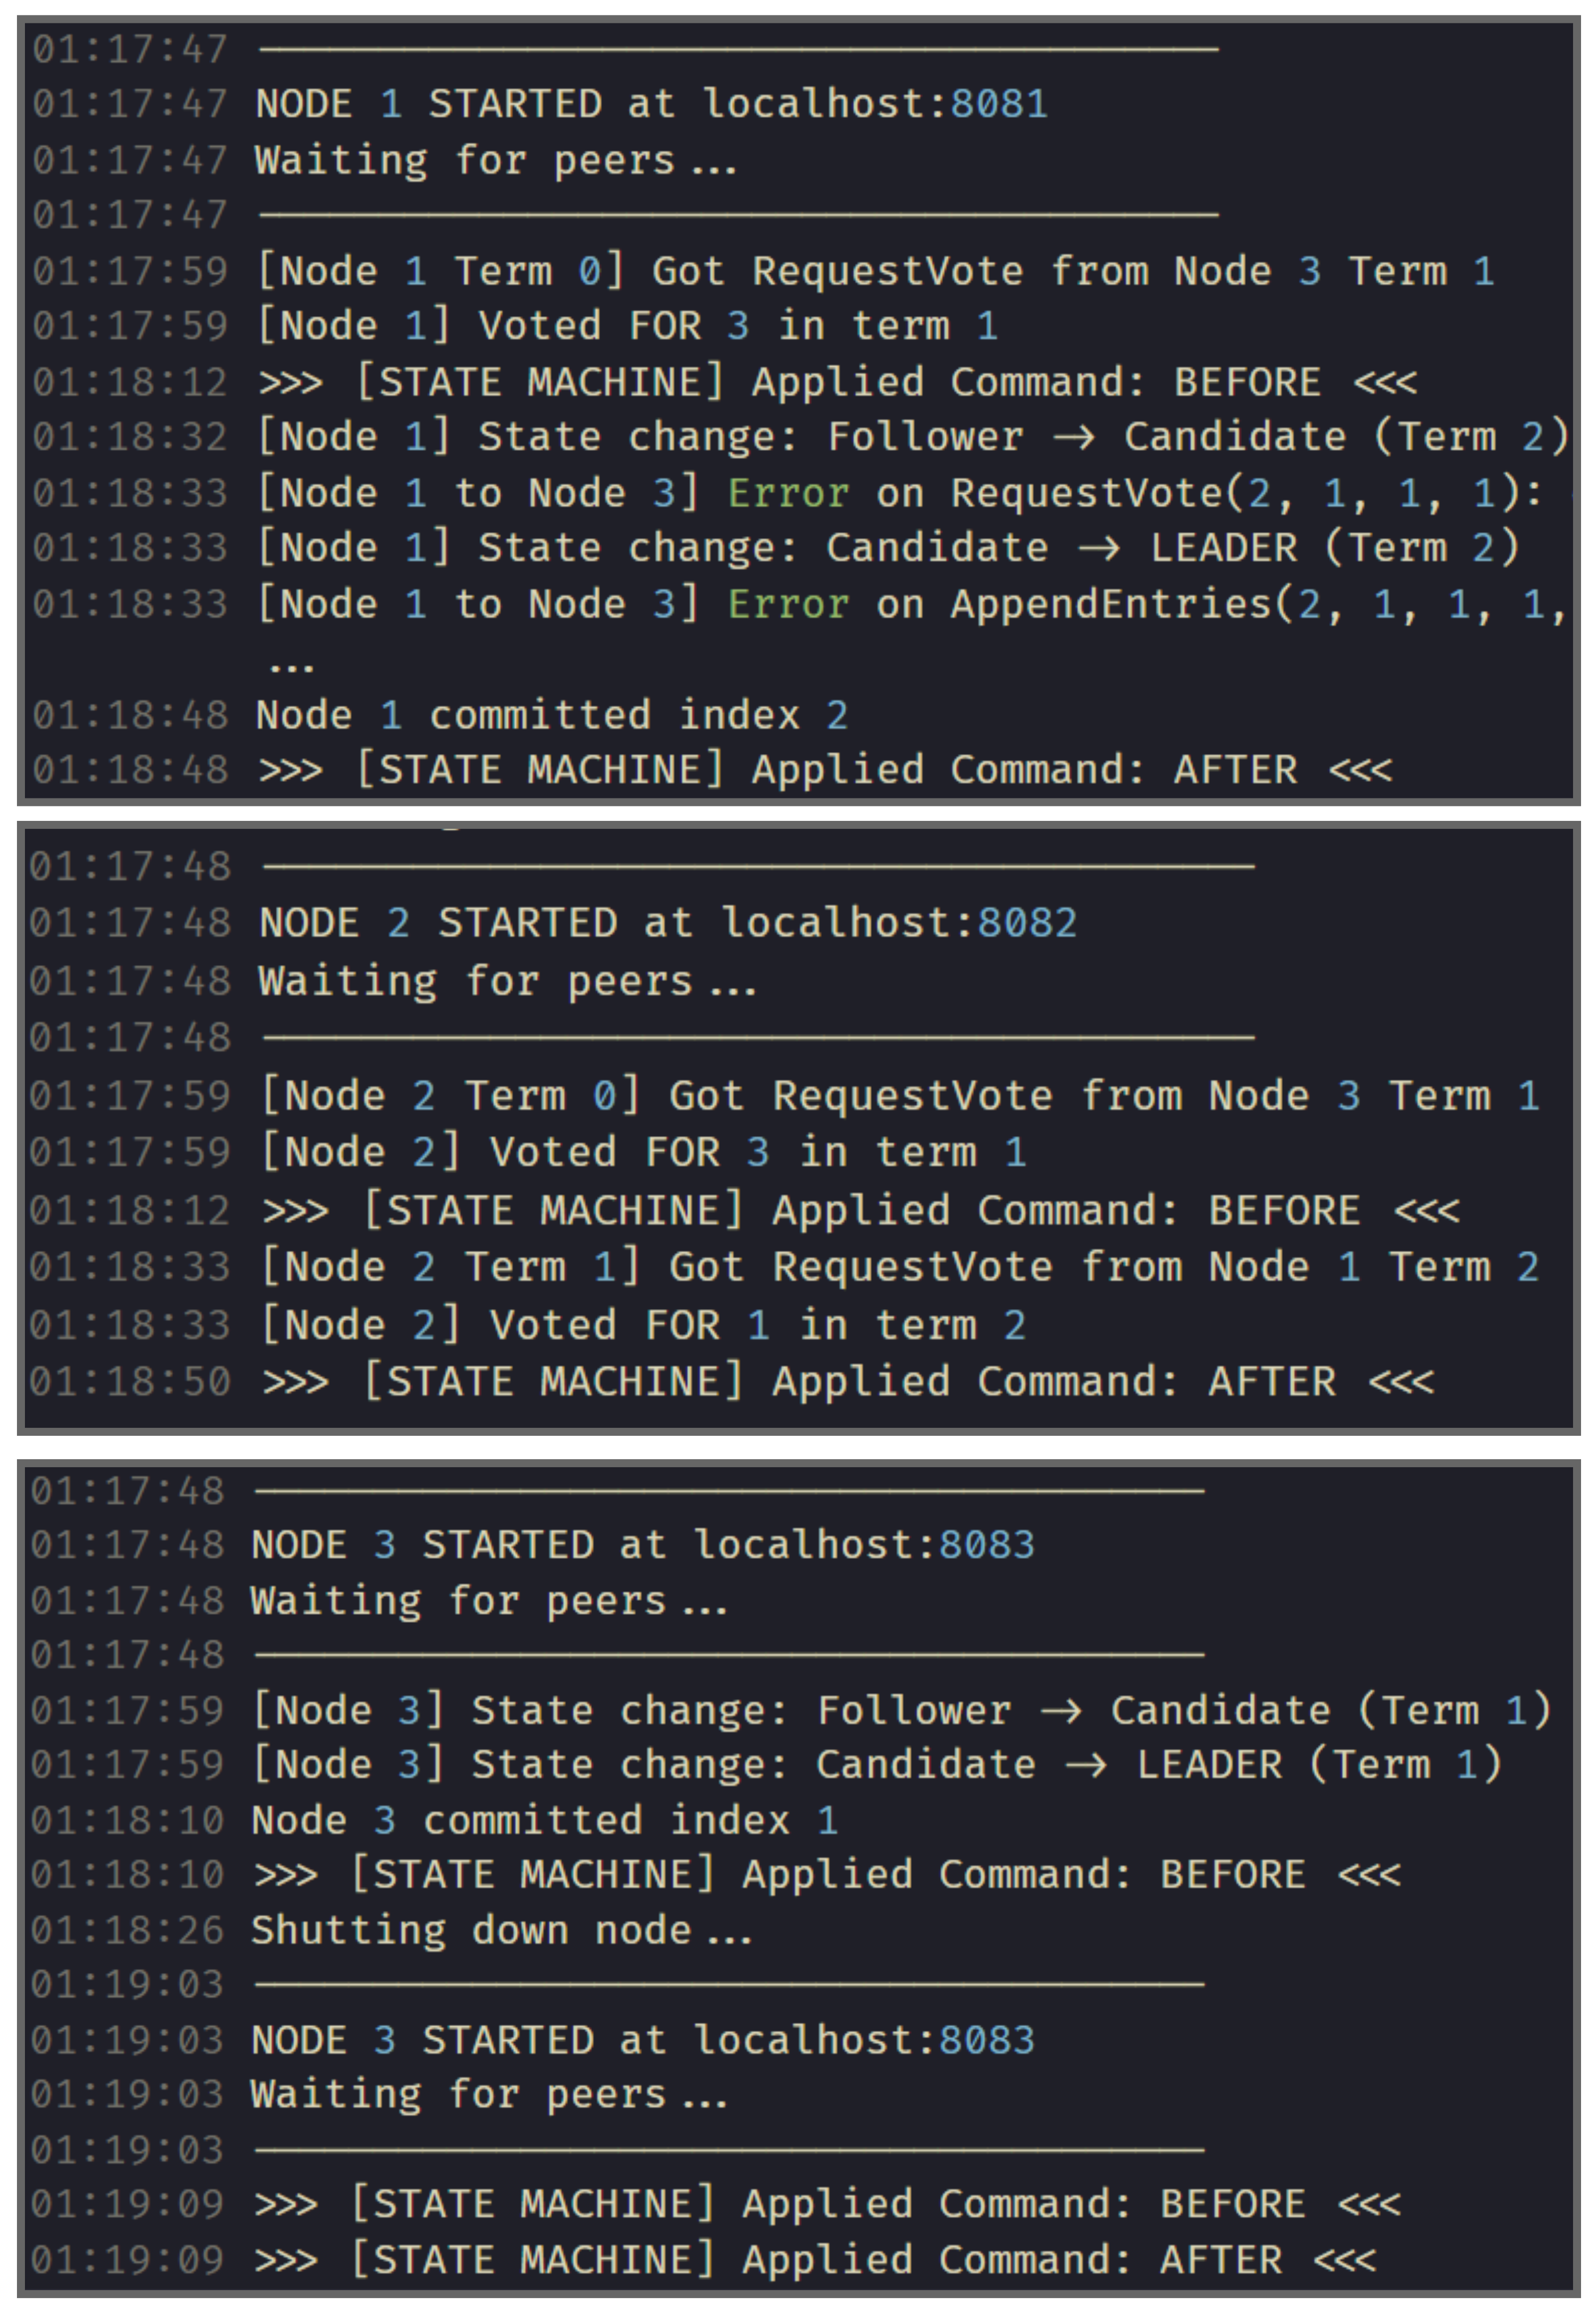
\includegraphics[width=0.9\textwidth]{images/tests/recovery.png}
    \caption{Скриншот логов: Реинтеграция узла и синхронизация данных}
    \label{fig:recovery}
\end{figure}
